\documentclass[11pt,varwidth=\maxdimen]{standalone}
%\documentclass{article}
\usepackage[english]{babel}	
\usepackage[utf8]{inputenc}	% Allows for writing special charachters in the tex-file 

\usepackage{amsfonts,amsmath,amssymb,bm,mathrsfs,mathtools,dsfont} 	% Standard mathematics 

\newcommand{\braces}[1]{\left\lbrace #1 \right\rbrace}
\newcommand{\brackets}[1]{\left( #1 \right)}
\newcommand{\squarebrackets}[1]{\left[ #1 \right]} 
\newcommand{\angles}[1]{\left\langle #1\right\rangle}
\newcommand{\abs}[1]{\left\lvert #1 \right\rvert}
\newcommand{\norm}[1]{\left\Vert #1 \right\Vert}

\usepackage[dvipsnames,table]{xcolor}
\definecolor{rmp}{RGB}{41, 43, 133}
\definecolor{myblue}{rgb}{0.24, 0.36, 0.44}
\definecolor{mygreen}{rgb}{0.367, 0.473, 0.0}
\newcommand{\myBlue}[0]{RoyalBlue}
\newcommand{\myGreen}[0]{OliveGreen}
\newcommand{\myRed}[0]{OrangeRed}
\newcommand{\myYellow}[0]{Goldenrod}


\usepackage{tikz}
\usepackage[compat=1.1.0]{tikz-feynman}
\usetikzlibrary{positioning,shapes,calc,arrows.meta}
\newcommand{\coord}[4]{({(#1)+(#3)*cos(#4)},{(#2)+(#3)*sin(#4)})}


\newcommand{\sscript}[1]{{\scriptscriptstyle \mathrm{#1}}}
\newcommand{\EFT}{\sscript{EFT}}


% % % % % % Commands % % % % % % %

\begin{document}

% Diagram 1
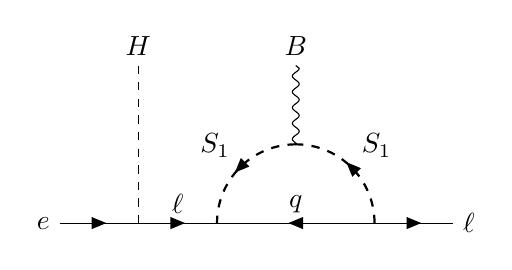
\begin{tikzpicture}
%\tikzset{baseline=(c.base)}
\tikzfeynmanset{inline=(e1.base)}
\begin{feynman}
	\vertex (a1);
    \vertex[left=1cm of a1] (e1) {$e$};
    \vertex[right=1cm of a1] (loop1);
    \vertex[right=2cm of loop1] (loop2);
    \vertex[right=1cm of loop2] (l1) {$\ell$};
    \vertex[above=2cm of a1] (h1) {$H$};
    \vertex[right=1cm of loop1] (aux1);
    \vertex[above=1cm of aux1] (loop3);
    \vertex[above=1cm of loop3] (w1) {$B$};
    
    \diagram*[baseline=(e1.base)] {
      {[edges=fermion]
        (e1) -- (a1) -- [edge label=$\ell$] (loop1),
        (loop2) -- [edge label'=$q$] (loop1),
        (loop2) -- (l1),
      },
      (loop2) -- [charged scalar,thick, quarter right, edge label'=$S_1$] (loop3) -- [charged scalar,thick, quarter right, edge label'=$S_1$] (loop1),
      % (loop1) -- [charged scalar,thick, edge label=$S_1$] (loop2),
      (h1) -- [scalar] (a1),
      (loop3) -- [boson] (w1),
    };

\end{feynman}
\end{tikzpicture} 

\end{document}